\section{Kernels within Kernels}

\begin{frame}
   {Kernel within Kernels}
   \begin{itemize}
      \item An introduction to:
      \begin{itemize}
         \item kvm
         \item libvirtd
         \item virsh
      \end{itemize}
   \end{itemize}

\end{frame}

\cprotect\note{

When we talk about kernel within kernels, we are looking to run an 
operating system as an application on an existing running computer. 
Perhaps we would like to run a copy of an old operating system
on a new piece of hardware, one the old operating system knows nothing 
about or we may require separate operating system environments for a 
specific application that doesn't get along with other applications. 
Whatever the reason we would like to have multiple operating systems 
running on a single platform. The tools we are going to look at 
to run our kernel within a kernel are: \textbf{kvm}, \textbf{libvirtd}
and \textbf{virsh}.  



}

\section{KVM}

\begin{frame}
   {KVM:  Kernel Virtual Machine}
   \begin{itemize}
      \item An open source virtualization technology built into Linux
      \begin{itemize}
         \item turns Linux into a hypervisor that allows virtual guests to be created
	 \item uses Linux for process management such as memory management, io, scheduling
         \item included in kernel version 2.6.20 and later
      \end{itemize}
      \item KVM uses Virtualization extensions in the processor chips
      \begin{itemize}
	      \item Intel: VT-x (also known as vmx) 
	      \item AMD: AMD-V (also known as svm) 
      \end{itemize}
   \end{itemize}

\end{frame}

\cprotect\note{

	The virtualization extensions may be disabled inn the BIOS
	of the computer, enable them as necessary. If the options are enabled
	they will be listed in the file \filelink{/proc/cpuinfo} in the \textbf{flags} list.
	Use a command like \textbf{grep -e svm -e vmx /proc/cpuinfo} to verify
	the kernel can see the extension flags. 

	These cpu extensions, \textbf{svm} and \textbf{vmx} are necessary for \textbf{KVM} but are
	not the only extensions to enhance virtualization. Some of the additional 
	\textbf{Intel} are:
	\begin{itemize}
		\item \textbf{EPT} Extended Page Tables
		\item \textbf{SR-IOV} Single Root I/O Virtualization
		\item \textbf{DDIO} Data Direct I/O Technology
	\end{itemize} 
	Virtualization enhancements exist in most processor chips, some examples can 
	be found at: 
	\begin{itemize} 
		\item AMD: \url{https://www.amd.com/en-us/solutions/servers/virtualization}
		\item Intel: \url{https://www.intel.ca/content/www/ca/en/virtualization/virtualization-technology/intel-virtualization-technology.html}
		\item ARM: \url{https://genode.org/documentation/articles/arm_virtualization/}
	\end{itemize}

}

\begin{frame}
	{KVM: the modules} 
	
	\textbf{KVM} is comprised of two kernel modules, a common module and 
	a processor specific module:
	\begin{itemize} 
		\item \textbf{kvm.ko} 
			\begin{itemize}
			\item common to all architectures
			\item provides the virtualization infrastructure
			\item accessible through the \textbf{kvm api}
			\end{itemize}

		\item \textbf{kvm-intel.ko} or \textbf{kvm-amd.ko}
			\begin{itemize}
			\item specific processor type module
			\item kernel driver module for specific hardware and related extensions.
			\end{itemize}
	\end{itemize}

\end{frame}

\cprotect\note { 

	There is an API interface available to use the \textbf{KVM} modules. The kvm api 
	is a set of \textbf{ioctls} to control components of a virtual machine.
	The ioctls fall into three classes: 
	\begin{itemize}
		\item System ioctls: used to query and set global kvm subsystem attribute's
		\begin{itemize}
			\item use this ioctl to create a virtual machine 
		\end{itemize}
		\item VM ioctls: used to query and set attributes 
			that affect a single virtual machine environment 
			\begin{itemize}
			\item  manipulate memory layout 
			\item  create virtual CPU's (vcpus)
			\end{itemize}
			\item vcpu ioctls: used to control the operation of a single vcpu.
			\begin{itemize}
			\item  run a guest virtual cpu 
			\end{itemize}
	\end{itemize}		
			
	See 
	\url{http://www.kernel.org/doc/Documentation/Virtual/kvm/api.txt} 
	for more information on the API or perhaps 
	\url{http://lwn.net/Articles/658511} for an example of 
	coding the API directly. 

	
}

\begin{frame}
   {QEMU: Quick Emulator, the glue}
   \begin{itemize}
	   \item Is a Virtual Machine Monitor (VMM) or Hypervisor
      \begin{itemize}
	 \item emulates various CPU's 
	 \item provides device models 
         \item executes as an emulator using dynamic binary translation 
         \item uses hardware virtualization extensions when coupled with KVM
      \end{itemize}
         \item The combination of QEMU and KVM with
		 hardware virtualization extensions can achieve near 
		 native performance within the VM's 
   \end{itemize}

\end{frame}

\cprotect\note{

   \textbf{QEMU} 
   brings configuration interface
   emulation of disk, nic, etc. Documentation on the various 
   devices that are emulated and their 
   options can be found in the 
   \textbf{QEMU Documentation} at:

   \url{https://www.qemu.org/documentation/}

   A discussion on \textbf{Understanding QEMU devices} is at: 
   
   \url{https://www.qemu.org/2018/02/09/understanding-qemu-devices/}.


}


\begin{frame}
   {kvm overview}
   \begin{figure}[H]
      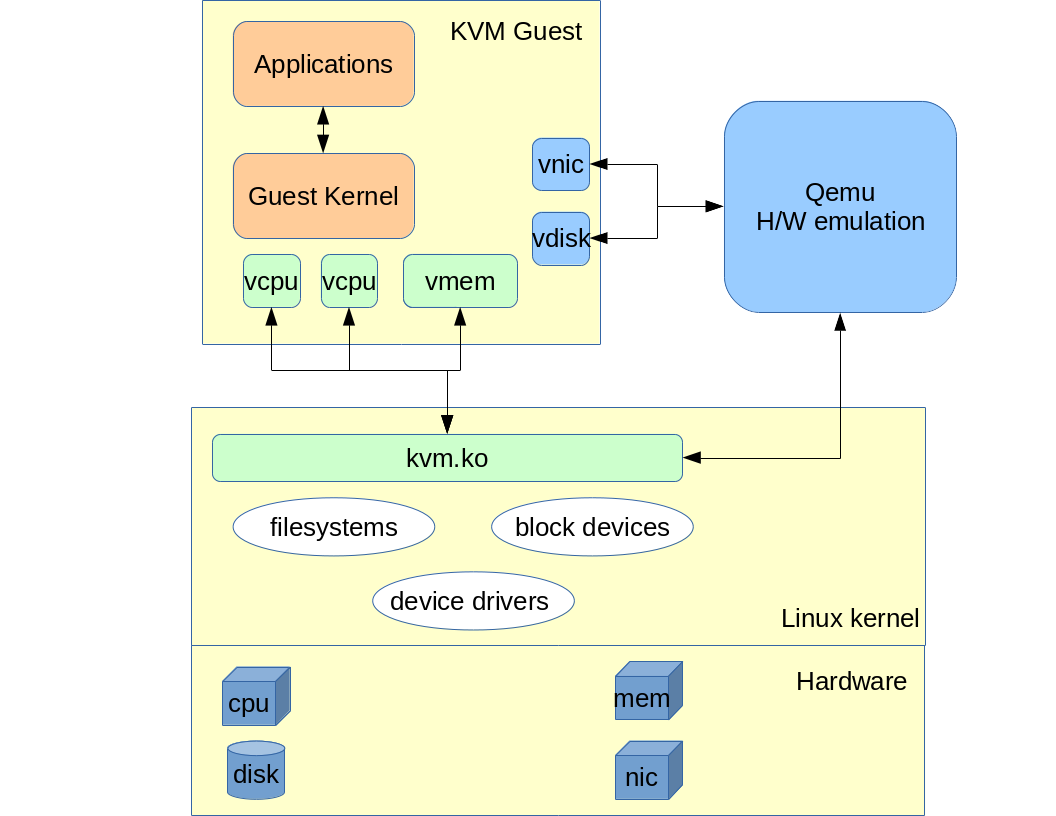
\includegraphics[height=3.2in]{IMAGES/kvm-over.png}
      \caption{Overview of kvm}
   \end{figure}
\end{frame}

\cprotect\note{

	The key to \textbf{KVM} actually running a virtual machine is a combination 
	of components. When these components are combined a fully functional virtual machine 
	capable of running an operating systems is created. The components are: 
	\begin{itemize}
		\item Kernel support and the two kernel modules
		\item Configuration method for the modules, the kvmapi 
		\item Something that looks like disk type storage, qemu
		\item Bootable loader, or bios provided by qemu 
		\item Additional virtual devices (NIC or Monitor) that link to the real devices, qemu
		\item A debug method, the qemu-monitor
	\end{itemize}

	The \textbf{KVM} kernel modules do the heavy work of securely managing the memory and cpu 
	requests from the VM's where as \textbf{qemu} provides the \textbf{VM's} with the peripheral 
	devices like virtual network cards, virtual storage devices and other virtual devices. 

}


\begin{frame}
	{KVM/QEMU configuration} 
		Configuring and starting a \textbf{VM} with \textbf{KVM/QEMU} can be done 
		at the command line. There are a few steps: 
	\begin{itemize}
		\item Confirm or load the appropriate \textbf{KVM} module
		\item Create an image file to be used as a disk 
		\item Start \textbf{qemu-kvm} with a list of options:
			\begin{itemize}
				\item disk image for storage
				\item disk (or image) of a CD-ROM to install from
				\item memory size directive
				\item a boot command
			\end{itemize}
		\item Install the operating system on the \textbf{VM}
		\item Stop the VM after the install is complete 
		\item Restart the VM like before but select the disk image to boot from
	\end{itemize}

\end{frame}


\cprotect\note{

	The commands to install and run a \textbf{VM} might look like this: 

	Create a 8G disk image
	\begin{raw}
# qemu-img create -f qcow2 vdisk.img 8G
	\end{raw}
	Boot from a CDrom image file, and install to the disk image
	\begin{raw}
# qemu-system-x86_64 -hda vdisk.img -cdrom /path/to/cdimage.iso -boot d -m 512
	\end{raw}
	When the install is complete restart the virtual machine without the CDrom
	\begin{raw}
# qemu-system-x86_64 vdisk.img -m 512
	\end{raw}
	
	This will start a \textbf{VM}, a very basic one, with no network and limited resources 
	but it will work. In order to meet the challenge of managing all these components, \textbf{libvirt} 
	was created. 



}	
